\documentclass{astroedu-lab}

\begin{document}

\pagestyle{plain}

\begin{problem}{\huge Лабораторная работа 2.4.1\\\\Измерение магнитного поля Земли\\\\Выполнил Жданов Елисей Б01-205}

\section{Цель работы:}

1) Определить характеристики шарообразных неодимовых магнитов 

2) Измерить горизонтальную и вертикальную составляющие индукции магнитного поля Земли и магнитное наклонение.

\section{Оборудование:}

Стеклянная газоразрядная трубка, наполненная неоном

Высоковольтный источник питания

Источник питания постоянного тока

Делитель напряжения

Резистор

Потенциометр

Амперметры

Вольтметры

Переключатели

\section{Теоретическая справка}

В данной работе рассматривается стационарные распределения Больцмана и остальных параметров.

Используя формулу потока частиц, можно получить полуэмпипическую формулу Бома

\begin{equation}
	I_\text{iн} = 0.4 n_e e S \sqrt{\frac{2 k T_e}{m_i}}
\end{equation}

Плазменная частота колебаний электронов выводится из уравнения колебаний среды

\begin{equation}
	\omega_p = \sqrt{\frac{4 \pi n_e e^2}{m_e}}
\end{equation}

Через такую плазму проходят частоты $\omega > \omega_p$, иные просто от нее отражаются.

Записав отношение скорости электронов к частоте, можно получить характерный масштаб, в котором не выполняется квазинейтральность плазмы

Таким образом, записав его для электронов и ионов, можно получить электронную поляризационную длину

\begin{equation}
	r_{De} = \sqrt{\frac{k T_e}{4 \pi n_e e^2}}
\end{equation}

и дебаевский радиус экранирования

\begin{equation}
	r_D = \sqrt{\frac{k T_i}{4 \pi n_e e^2}}
\end{equation}

Среднее же число ионов в дебаевской сфере

\begin{equation}
	N_D = \frac{4}{3} \pi r_D^3 n_i
\end{equation}

Наконец, степень ионизации плазмы

\begin{equation}
	\alpha = \frac{n_i}{n}
\end{equation}

\section{Экспериментальная установка}

\begin{figure}[!h]
	\centering
	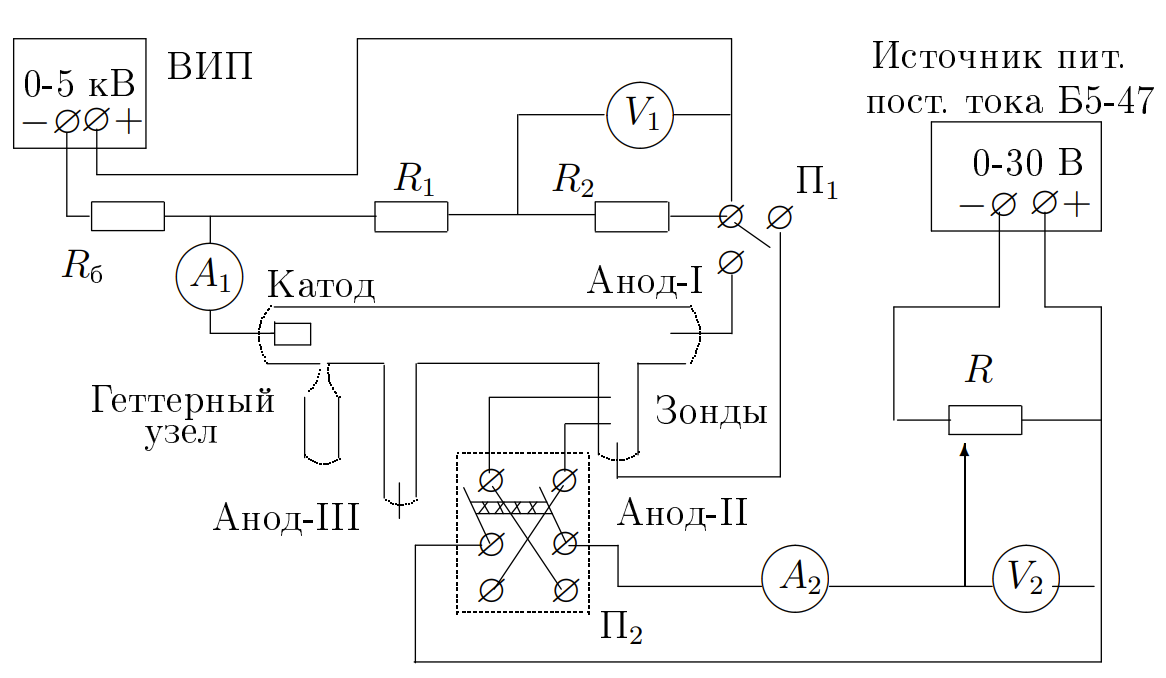
\includegraphics[width=0.9\textwidth]{установка.png}
	\label{fig:boiler}
\end{figure}

Схема установки для исследования плазмы газового разряда в неоне представлена на рисунке. Стеклянная газоразрядная трубка
имеет холодный (ненагреваемый) полый катод, три анода и геттерный узел стеклянный баллон, на внутреннюю поверхность которого напылена газопоглощающая плёнка (геттер). Трубка наполнена изотопом неона $^{22}$Ne при давлении 2 мм рт. ст.

Катод и один из анодов (I или II) с помощью переключателя П$_1$ подключаются
через балластный резистор R$_\text{б}$ (450 кОм) к регулируемому высоковольтному
источнику питания (ВИП) с выходным напряжением до 5 кВ.

При подключении к ВИП анода-I между ним и катодом возникает газовый разряд. Ток разряда измеряется миллиамперметром A$_1$, а падение напряжения на разрядной трубке цировым вольтметром V$_1$ (мультиметром GDM), подключённым к трубке через высокоомный (25 МОм) делитель напряжения с коэициентом (R$_1$ + R$_2$)/R$_2$ = 10.

При подключении к ВИП анода-II разряд возникает в про
транстве между катодом и анодом-II, где находится двойной зонд, используемый для диагностики плазмы положительного столба.

Зонды изготовлены из молибденовой проволоки диаметром d = 0.2 мм и имеют длину l = 5.2 мм. Они подключены к источнику питания GPS через потенциометр R. Переключатель П$_2$ позволяет изменять полярность напряжения на зондах. Величина напряжения на зондах изменяется с помощью дискретного переключателя V выходного напряжения источника питания и потенциометра R, а измеряется цировым вольтметром V$_2$ (GDM). Для измерения зондового тока используется
мультиметр A$_2$ (GDM). Анод-III в нашей работе не используется.

\section{Измерения, Обработка}

При обработке считается, что доминирующий вклад в погрешность вносит случайный разброс величин, а погрешностью измерения приборов можно пренебречь(что в результате будет очевидно).

Вольт - амперная характеристика разряда и теоретический график ВАХ

\newpage

\begin{figure}[!h]
	\centering
	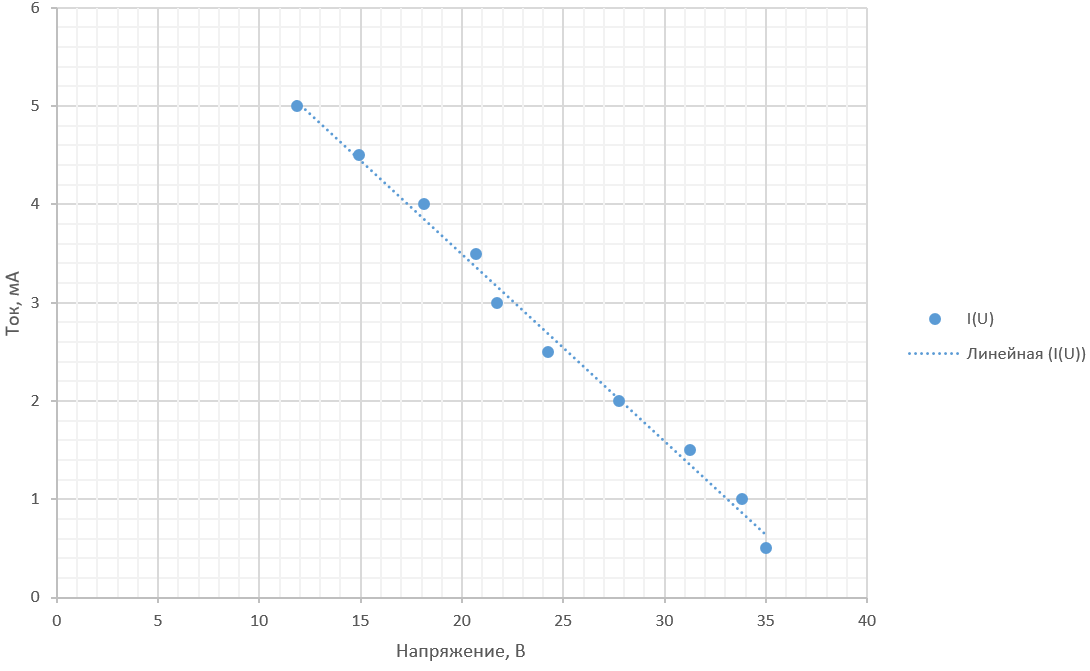
\includegraphics[width=0.9\textwidth]{вах.png}
	\label{fig:boiler}
\end{figure}

\begin{figure}[!h]
	\centering
	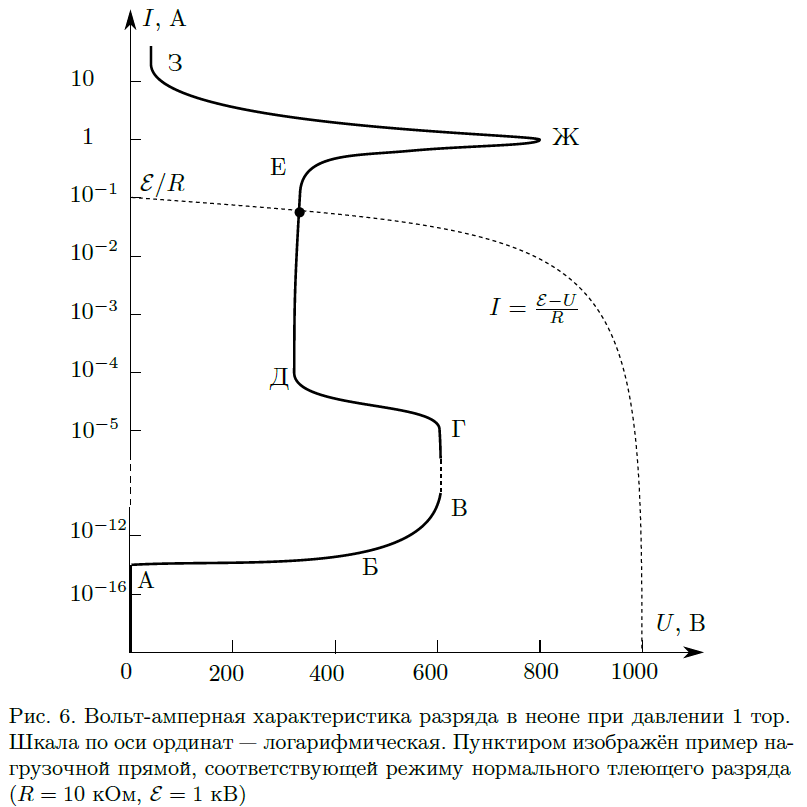
\includegraphics[width=0.9\textwidth]{th1.png}
	\label{fig:boiler}
\end{figure}

\newpage

Найдем угловые коэффициент ВАХ по МНК.

\begin{equation}
	y = (7.3 \pm 0.15) - (0.1902 \pm 0.0061) \cdot x
\end{equation}

\[
	a = \frac{<x_i y_i> - < x > < y_i >}{< x_i^2> - < x_i >^2}
\]

\[
	b = < \nu_i > - a < N_i >
\]

Также рассчитаем их погрешности

\begin{equation}
	S_a^2 = \frac{< x_i^2>}{< x_i^2 > - < x_i >^2} \cdot \frac{<  b_i - b > ^2}{n - 2}
\end{equation}

Итого $R_\text{диф} = \frac{dU}{dI} = \frac{1}{a} = -5.26 \pm 0.16 \text{ Ом}$

Как видим, поскольку наклон ВАХ отрицательный, сопротивление того же знака.

Очевидно, что ВАХ соответствует теоретическому участку ГД, правда ток в рассматриваемой установке значительно выше.

Графики зондовых характеристик


\newpage

\begin{figure}[!h]
	\centering
	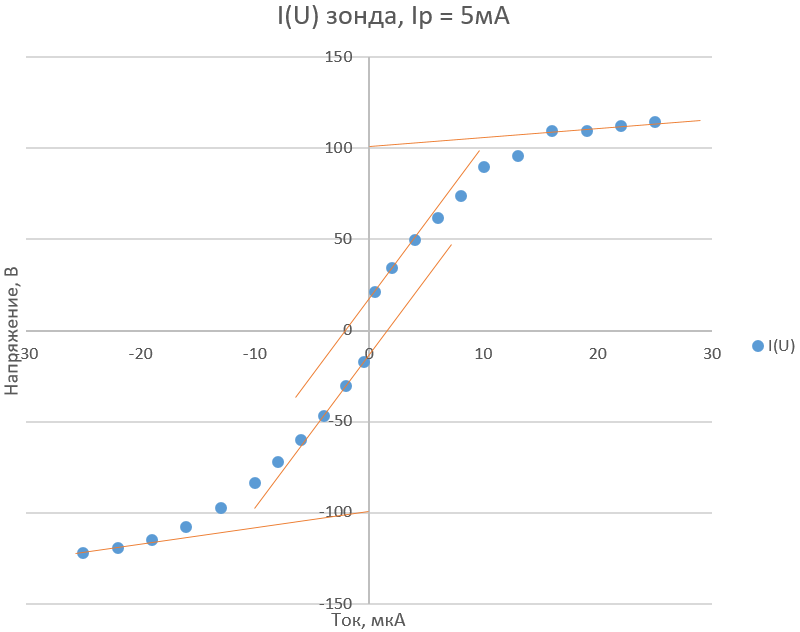
\includegraphics[width=1\textwidth]{5.png}
	\label{fig:boiler}
\end{figure}

\newpage

\begin{figure}[!h]
	\centering
	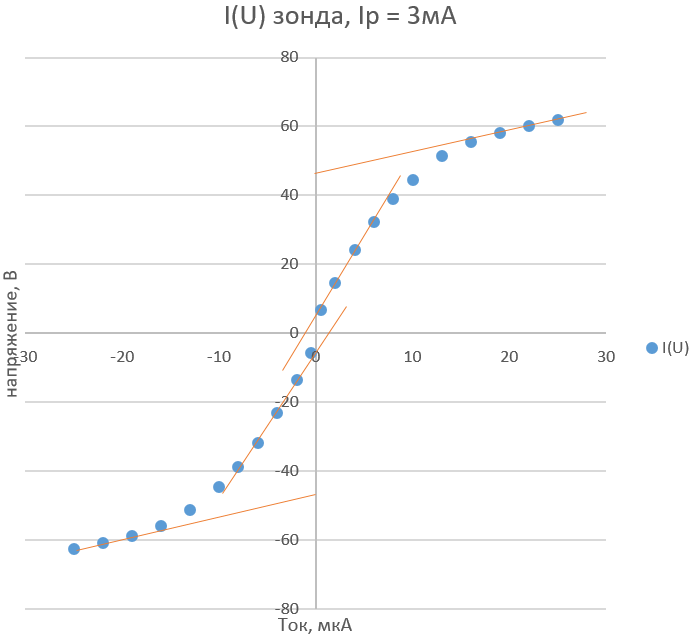
\includegraphics[width=1\textwidth]{3.png}
	\label{fig:boiler}
\end{figure}

\newpage

\begin{figure}[!h]
	\centering
	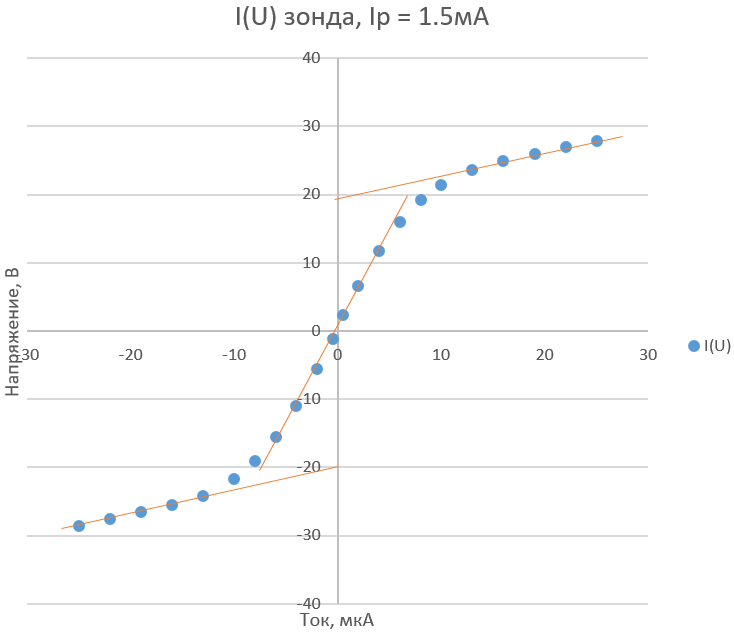
\includegraphics[width=1\textwidth]{1.5.png}
	\label{fig:boiler}
\end{figure}

\newpage

При помощи МНК построим требуемые асимптоты и касательные, получив необходимые значение, которые сведены в таблицу. Добавим расчет $\Delta U$

\begin{center}
\begin{tabular}{|c|c|c|c|}
\hline 
$I_p$, мА & $I_{\text{iн}}$, мкА & $\frac{dI}{dU}_{U=0}$ & $\Delta U$, В \\
\hline
$5$ 	& $(93 \pm 3)$ & $(8.2 \pm 0.4)$ & $(11.3 \pm 1.0)$ \\
$3$ 	& $(46.8 \pm 0.6)$ & $(4.95 \pm 0.12)$ & $(9.5 \pm 0.4)$ \\
$1.5$ 	& $(20.23 \pm 0.13)$ & $(2.74 \pm 0.11)$ & $(7.4 \pm 0.4)$ \\
\hline
\end{tabular}
\end{center}

Рассчитаем все требуемые величины в следующей таблице на основе $\Delta U$.

\begin{center}
\begin{tabular}{|c|c|c|c|c|c|c|c|}
\hline 
$I_p$, мА & $\Delta U$, В & $kT_e$, эВ & $T_e$, $10^3$К & $n_e$, $10^{16}$м$^{-3}$ & $\omega_p$, $10^{9}$ $\frac{\text{рад}}{\text{сек}}$ & $r_{De}$, мкм & $r_D$, мкм \\
\hline
$5$ 	& $11.3 \pm 1.0$ 	& $5.6 \pm 0.5$ & $67 \pm 6$ & 
$6.3 \pm 0.5$ & $14.2 \pm 0.6$		& $70 \pm 6$ & 
$4.8 \pm 0.2$ \\
$3$ 	& $9.5 \pm 0.4$ 	& $4.8 \pm 0.2$ & $56 \pm 2$ & 
$3.45 \pm 0.11$ & $10.48 \pm 0.17$	& $88 \pm 3$ & 
$6.44 \pm 0.11$ \\
$1.5$ 	& $7.4 \pm 0.4$ 	& $3.7 \pm 0.2$ & $44 \pm 2$ & 
$1.68 \pm 0.05$ & $7.31 \pm 0.11$	& $110 \pm 5$ & 
$9.22 \pm 0.14$ \\
\hline
\end{tabular}
\end{center}

\begin{center}
\begin{tabular}{|c|c|c|}
\hline 
$I_p$, мА & $N_D$ & $\alpha$, $10^{-7}$ \\
\hline
$5$ 	& $29 \pm 6$ & $9.8 \pm 0.8$ \\
$3$ 	& $39 \pm 3$ & $5.36 \pm 0.17$ \\
$1.5$ 	& $55 \pm 4$ & $2.61 \pm 0.08$ \\
\hline
\end{tabular}
\end{center}

Поскольку $r_{De}$ много меньше миллиметра, что все еще много меньше её линейных размеров, плазму можно считать квазинейтральной.

Число Дебая также довольно большое по сравнению с единицей, поэтому плазму можно рассматривать как идеальный газ.

Следовательно, все теоретические выкладки оправданны, и эксперимент можно считать корректным.

Построим графики $T_e\left(I_p\right)$ и $n_e\left(I_p\right)$

\newpage

\begin{figure}[!h]
	\centering
	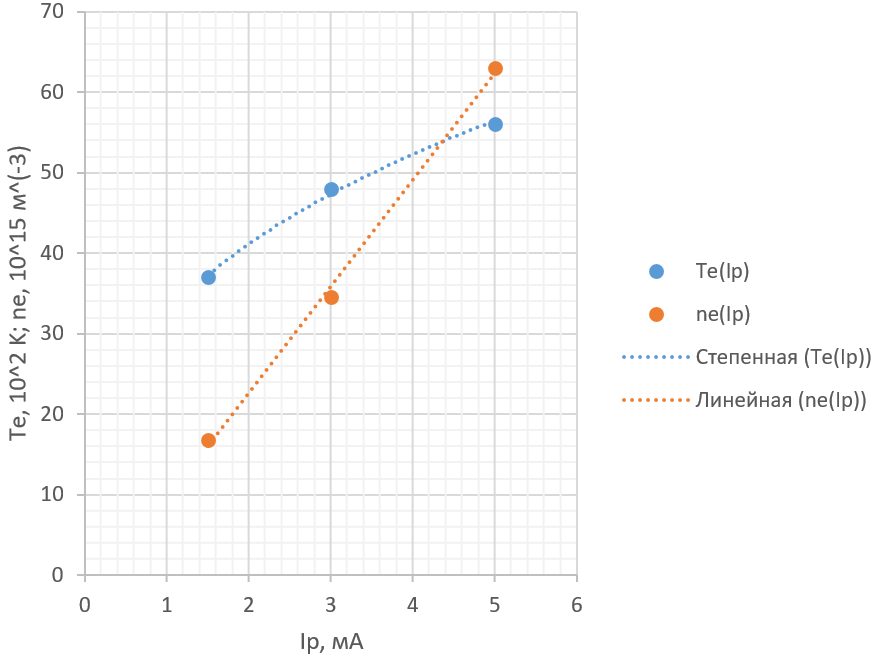
\includegraphics[width=1\textwidth]{ple.png}
	\label{fig:boiler}
\end{figure}

Собственно говоря, на приведенных графиках ничего нового не наблюдается - температурная зависимость аппроксимируется коренной функцией $\sqrt{x}$, а зависимость концентрации прямо пропорциональна. Это замечательно согласуется с уже приведенными теоретическими выкладками

\section{Вывод}

В данной работе было исследовано множество характеристик тлеющего разряда в неоне при пониженном давлении. Фактически все полученные значения величин обладают небольшой погрешностью, лежат в рамках предположений и представляют собой хорошие характерные значения плазмы с точки зрения физики.

Отдельно хочется упомянуть графики I(U) зонда, на которых наблюдается разрыв в районе нуля. Это связано с некоторым холостым током в схеме, который по хорошему должнен быть исключен из графика. Тем не менее, на расчет коэффициентов и $\Delta U$ он повлиять не может.

\section{Ресурсы}

Расчет по МНК: метод-наименьших-квадратов.рф


\end{problem}
\end{document}